\section{Linear complexity RPE
implementation}

In this section we will detail how the relative positional encoding
 proposed by \citet{shaw2018selfattention}
can in fact be computed with linear complexity. The $S_{rel}$ matrix of scores is computed as
${S_{rel}}_{ij} = \vec{Q_i} \cdotp \vec{RP}_{clip(i-j, -k, k)}$. In figure \ref{fig:S_rel} the colors represent the index of the query and the number the
index of the relative position.

\begin{figure}
\centering
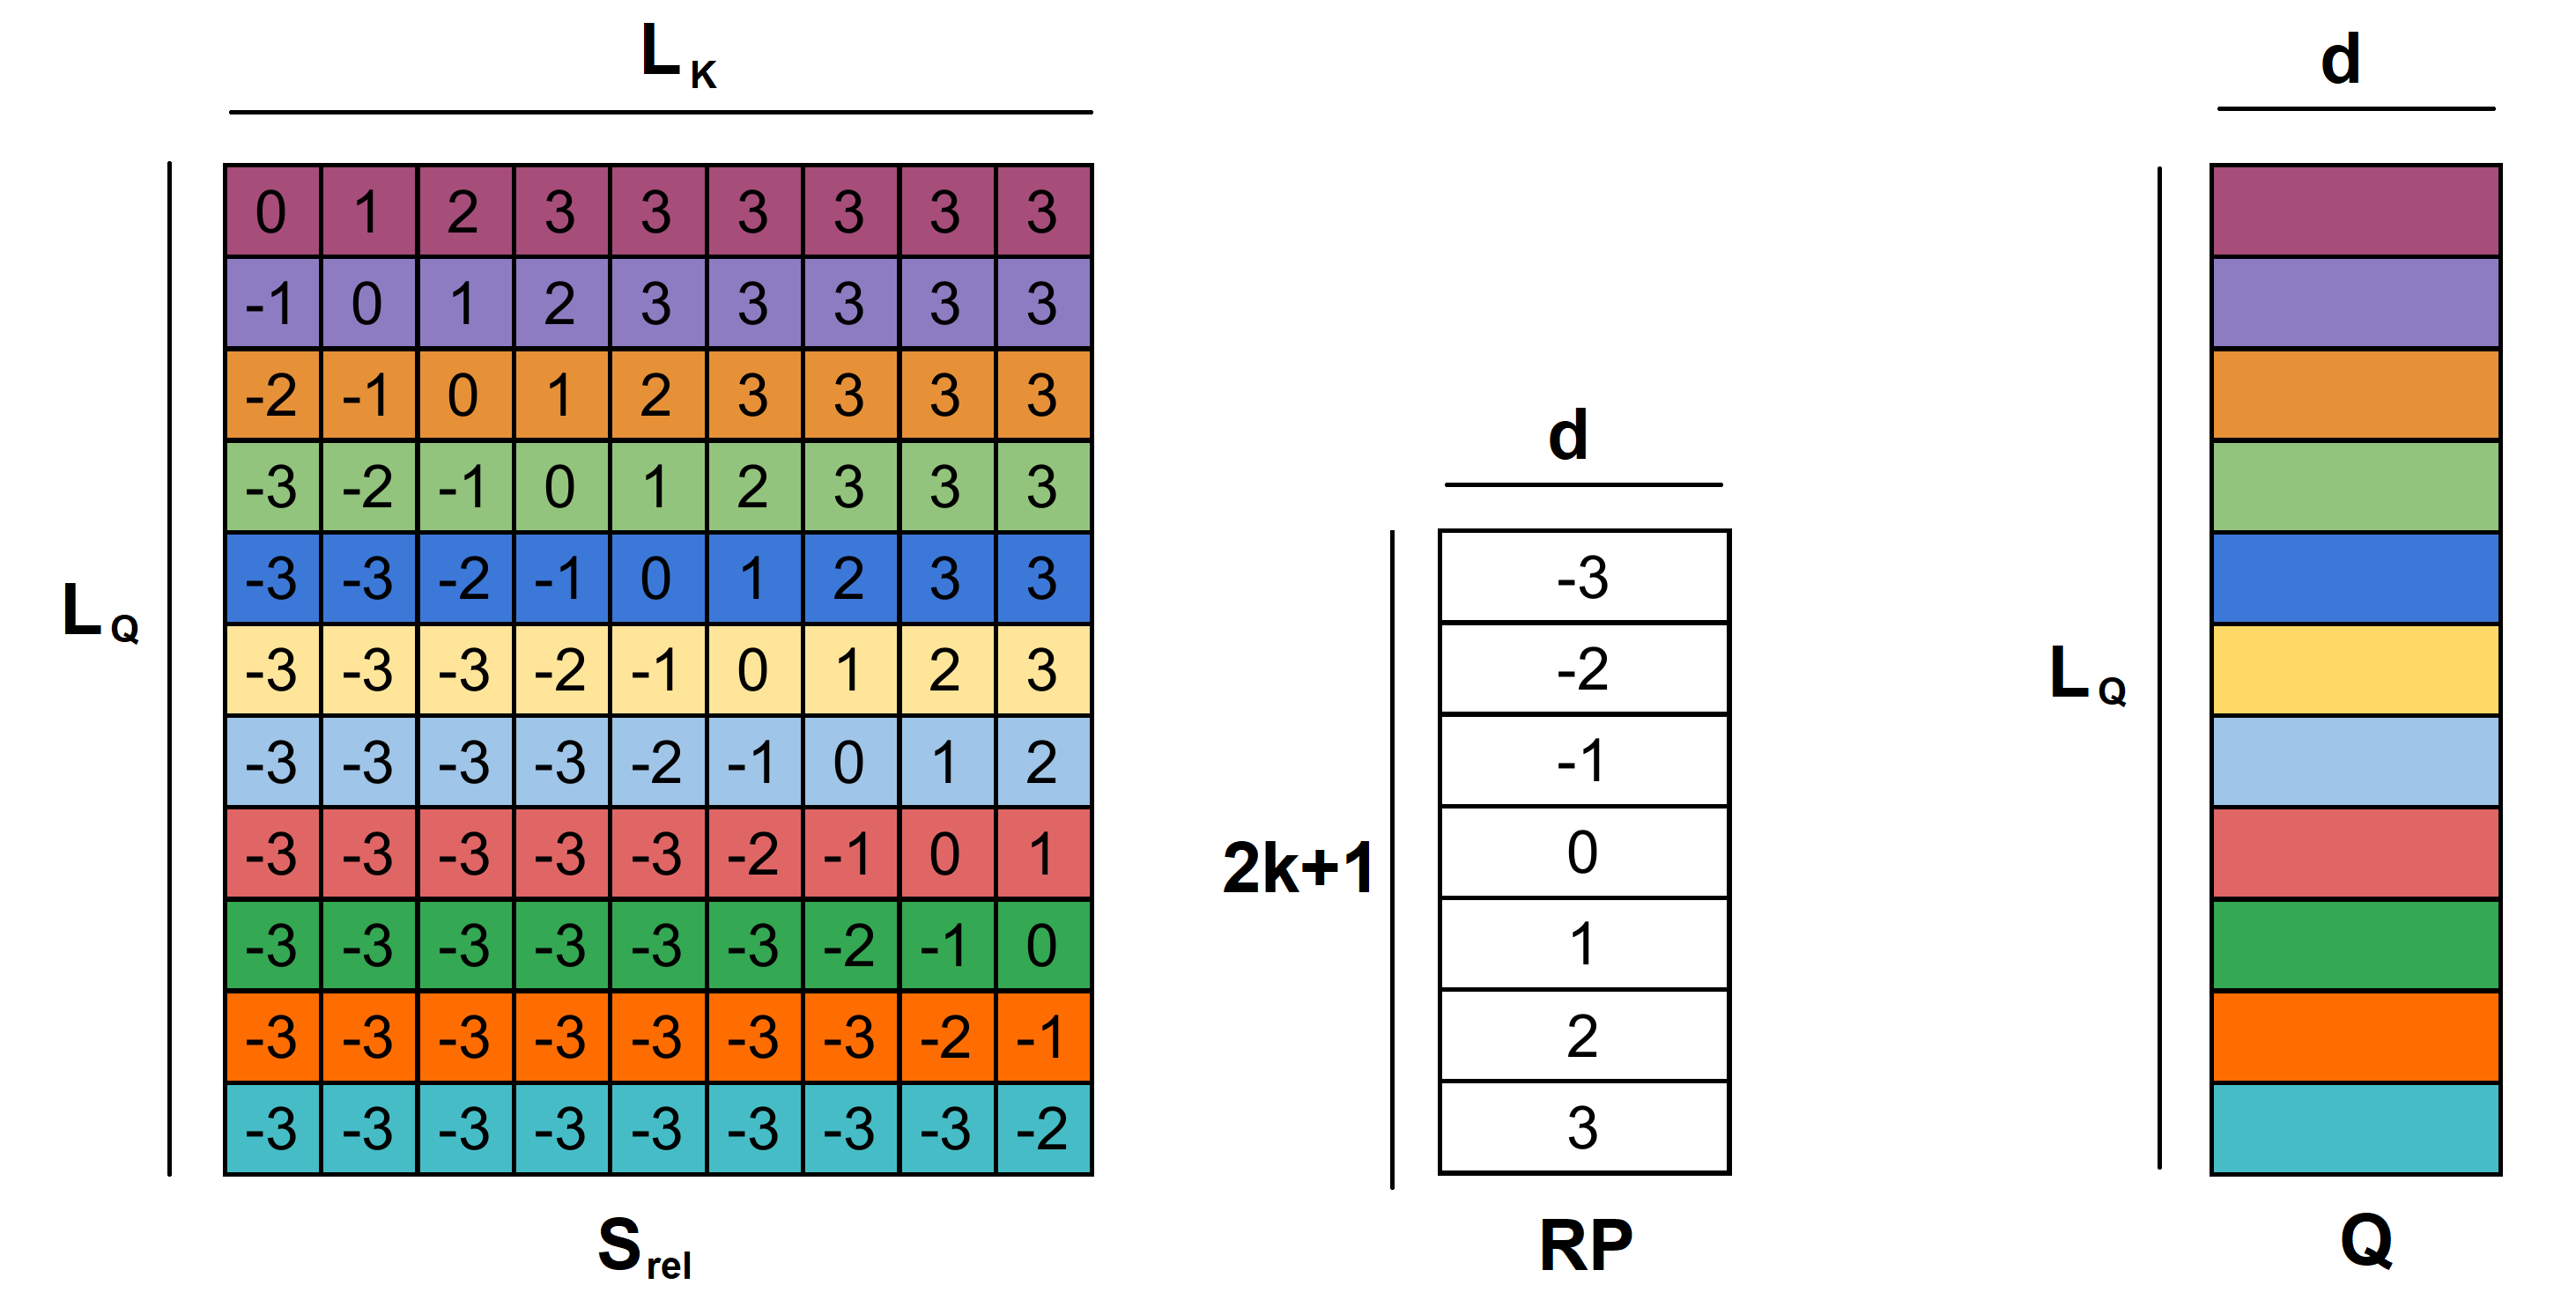
\includegraphics[width=0.9\linewidth]{images/S_rel.png}
\caption{$S_{rel}$ calculation}
\label{fig:S_rel}
\end{figure}

Finally we calculate $A_{rel} = S_{rel} \times V$. Each row of the $A_{rel}$ matrix is a weighted sum of the value vectors $V_i$. Each row of $S_{rel}$ is a set of weights.

\begin{figure}
\centering
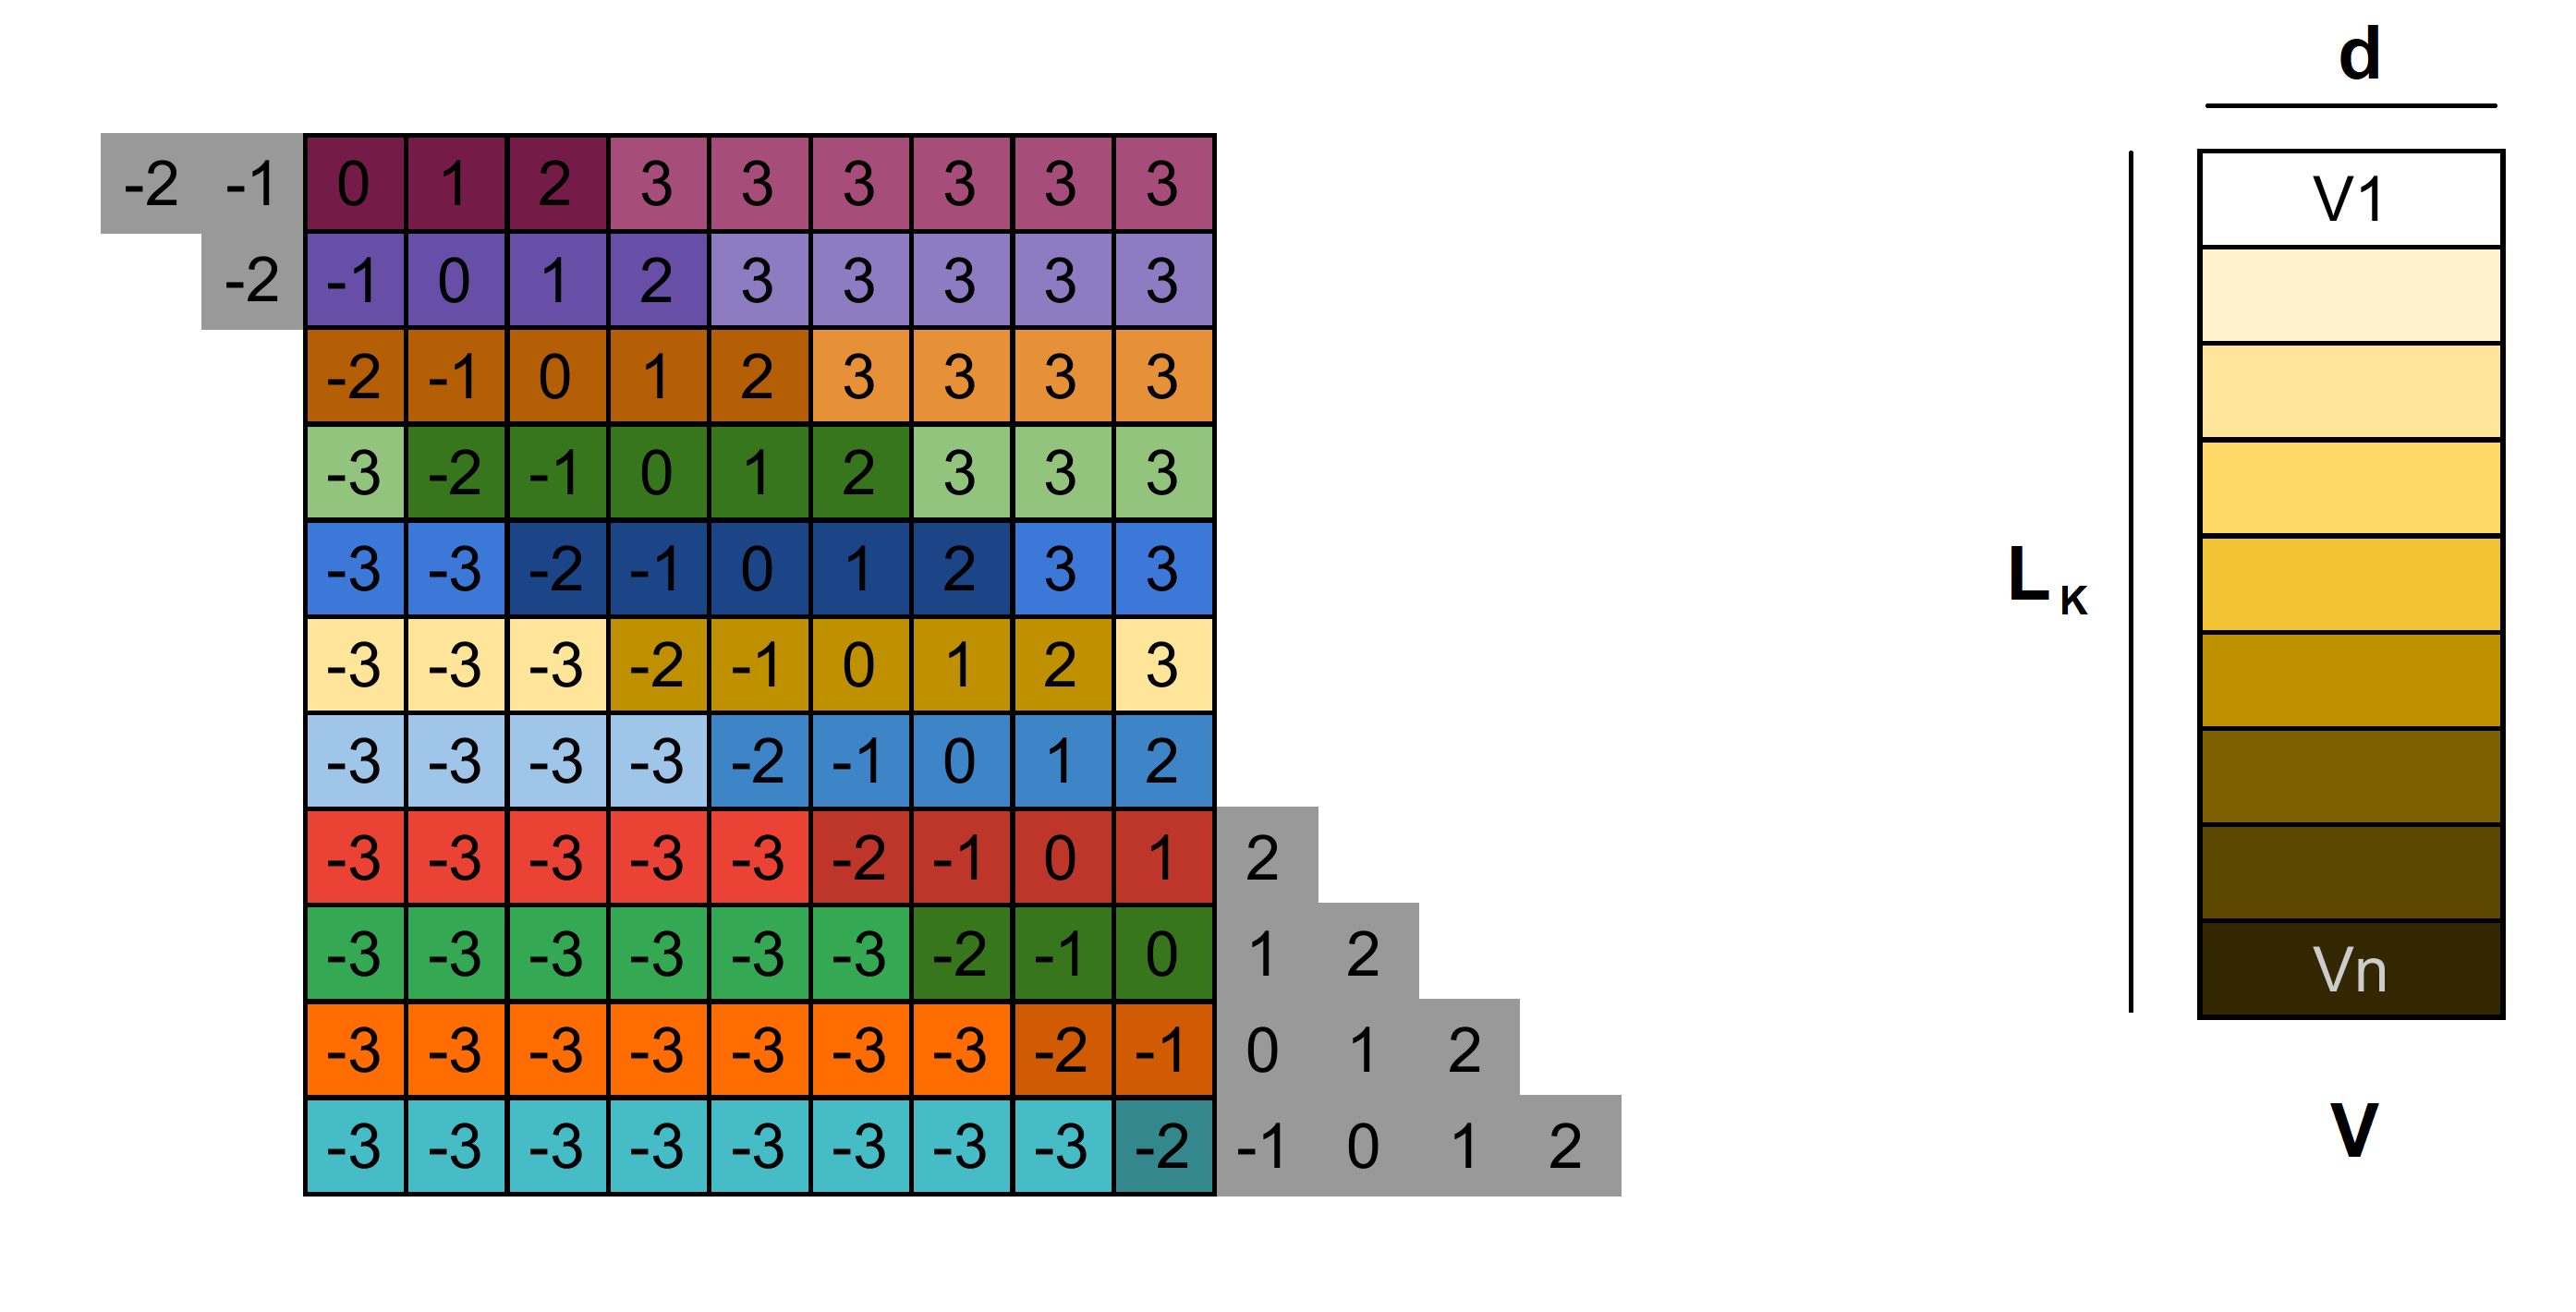
\includegraphics[width=0.9\linewidth]{images/S_rel_V.png}
\caption{$A_{rel}$ calculation}
\label{fig:A_rel_naive}
\end{figure}

One can observe in figure \ref{fig:A_rel_naive} that some weights are repeated several times in the
$S_{rel}$ matrix. Calculating the whole matrix can be avoided by
instead calculating all possible weights only once, with complexity
$O \left(L_Q\times d\times(2k+1)\right)$). As illustrated in figure \ref{fig:A_rel_linear}, the matrix multiplication can then be
replaced by a sum of three terms:

\begin{itemize}
\item A set of weights that multiply a
accumulated sum of value vectors (complexity $O(max(L_Q, L_K))$)
\item An
element-wise multiplication between two tensors (complexity
$O(L_Q\times (2k-1) \times d)$)
\item A set of weights that multiply a
accumulated sum of value vectors (complexity $O(max(L_Q, L_K))$).
\end{itemize}

\begin{figure}
\centering
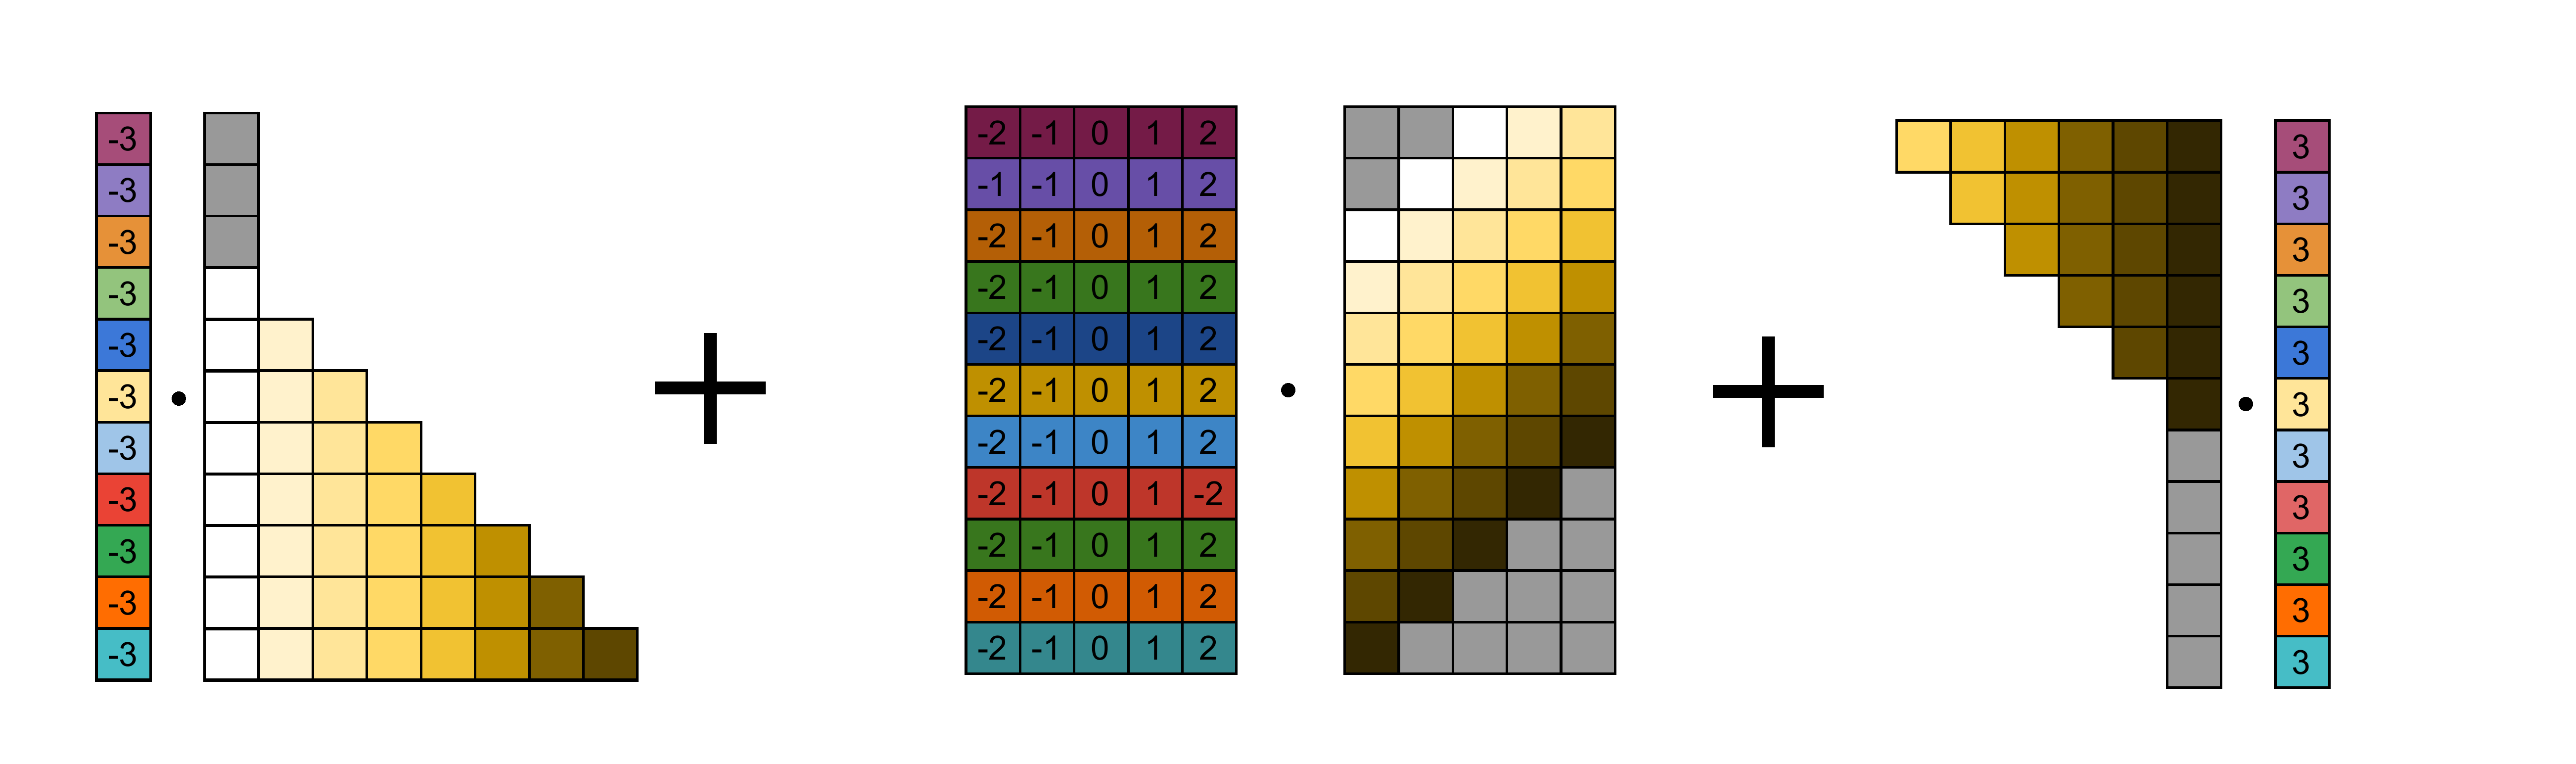
\includegraphics[width=0.9\linewidth]{images/S_rel_V_detailed.png}
\caption{$A_{rel}$ simplified calculation}
\label{fig:A_rel_linear}
\end{figure}

Thus the attention can in fact be computed with linear complexity if we
get rid of the softmax function.

The memory used can be further reduced by observing that the right side
of the second element is a strided view of a padded copy of the value
matrix. Moving of one cell along the first dimension is equivalent to
moving along one cell of the second dimension.

The calculation can be implemented as follow, using zero-based slice
notation for compactness:

\begin{itemize}
	\item
	$\phi(Q)$, $\phi(V)$ and $RP$, are matrices of shape
	$(L_Q, d)$, $(L_K, d)$ and $(2k+1, d)$ respectively
	\item
	The dot product of each query and each relative position embedding is
	calculated as $weights = \phi(Q) \times RP^T$
	\item
	The weights of the horizon before and after are
	$H_{before} = weights_{[:, 0]}$ and
	$H_{after} = weights_{[:, -1]}$
	\item
	The weights of the diagonal are defined as
	$window = weights_{[:,1:-1]}$. For the masked case, columns on the
	right of the $k^{th}$ columns are set to 0
	($window_{[:, k+1:]} = 0$)
	\item
	The left term is calculated as
	$left = H_{before} * align(lower, min(max(0, L_Q-k), L_K))$ with
	$lower$ the concatenation of:
	
	\begin{itemize}
		\item
		a tensor of zeros of shape $\left(min(k, L_Q), d\right)$
		\item
		$cumsum(V, dim=0)$
	\end{itemize}
	\item
	The middle term is calculated as $middle = diagonal \odot strided$
	with $strided$ the strided view of:
	
	\begin{itemize}
		\item
		a tensor of 0 of shape $(max(0, k-1), d)$
		\item
		the value matrix $V$
		\item
		a tensor of shape $(max(0, L_Q-L_K), d)$
	\end{itemize}
	\item
	The right term is calculated as $right = 0$ for masked case, or for
	bidirectional case, $right = H_{right} * reverse$, with reverse the
	concatenation of:
	
	\begin{itemize}
		\item
		a tensor of 0 of shape $(L_Q-max(0, L_K-k), d)$
		\item
		$sum(V_{[inf, sup]}, dim=0) - cumsum(V_{[inf, sup-1]}, dim=0)$
		with $inf = k-1$, $sup = min(L_Q+k, L_K)$
	\end{itemize}
	\item
	The resulting attention function is $A = left + middle + right$
\end{itemize}

with:

\begin{itemize}
	\item
	$*$ the element-wise multiplication
	\item
	$\odot$ the element-wise multiplication followed by sum along second
	dimension
	\item
	all concatenations done along the first dimension
\end{itemize}

\endinput
